% Architecture draft, revised 2026-10-23.
% Target architecture: femu_docker, CPU CSFs, application-controlled SNIA batches.
% Reference measurements and remaining result slots: DRAFT_NOTES.md.
\documentclass[sigconf, nonacm]{acmart}
%%% do not modify the following VLDB block %%
%%% VLDB block start %%%
\usepackage{pvldb}
%%% VLDB block end %%%
\usepackage{amsmath}
\usepackage{tikz}
\usetikzlibrary{arrows.meta,positioning,fit,calc}
\renewcommand\vldbdoi{XX.XX/XXX.XX}
\renewcommand\vldbpages{XXX-XXX}
\renewcommand\vldbavailabilityurl{}
\newcommand{\sys}{\textsc{CoSQL}}
\newcommand{\host}{\mathsf{H}}
\newcommand{\csd}{\mathsf{D}}
\newcommand{\pending}{\textemdash}
\begin{document}
\title{CoSQL: Composable SQL Offloading with Cache Refill on Computational Storage}
% Working system name; replace authors and publication metadata before submission.
\author{Anonymous Author(s)}
\renewcommand{\shortauthors}{Anonymous Author(s)}

\begin{abstract}
Computational storage reduces data movement by executing query operators near
stored data. Integrating this capability into a relational database requires
more than predicate pushdown: applications need a portable execution interface,
complete operator chains must run within limited device memory, and offloaded
scans should preserve opportunities to warm the host cache. These capabilities
also change where subsequent operators should execute. We present \sys{},
a PostgreSQL-based architecture that connects four mechanisms. A SNIA
Computational Storage API implementation exposes device memory, computation,
and batch dependencies through a common application interface. CPU-based
storage functions implement scans, joins, aggregation, and external sorting,
while the application composes their execution and manages dataflow. An NVMe
asynchronous-event protocol identifies scanned ranges for host cache refill
through ordinary reads. A bottom-up dynamic program chooses execution
locations using operator cost, device memory, result transfer, and observed
host cache residency. We organize evaluation around Host-only, Filter-only,
CSD-only, CSD + Cache Refill, and the full system to separate operator coverage,
cache reuse, and placement benefits. Preliminary SF=1 results provide reference
points for the evaluation; the design emphasizes the interaction between
composable offloading and host cache reuse across queries.
\end{abstract}
\maketitle
%%% do not modify the following VLDB block %%
%%% VLDB block start %%%
\vldbtopmatter
%%% VLDB block end %%%

\section{Introduction}
Analytical queries often move large volumes of data from storage to host
memory before discarding most of those bytes through filtering, joining, or
aggregation. Computational storage places processing resources beside the
data, allowing a database to exchange compact results rather than entire
inputs. Predicate pushdown is a natural starting point: scanning and filtering
near storage can reduce host-interface traffic without moving the rest of the
query engine. However, the output of a filter can still be large, and joins,
grouping, DISTINCT, and sorting can dominate the remaining work.

Existing systems demonstrate several steps beyond this starting point.
Ibex integrates selection, projection, and GROUP BY into an intelligent
storage engine \cite{ibex}. PushdownDB studies relational computation over
the restricted interface of S3 Select \cite{pushdowndb}. FlexPushdownDB
combines cached data and pushed-down computation using separable operators
\cite{fpdb}. These results establish both the value of near-data execution
and the importance of coordinating it with caching. Our question is how to
bring these ideas together for a locally attached, programmable CSD through
a standard application interface, while supporting complete analytical
operator chains and actively replenishing the host's cache.

We identify four connected gaps. \emph{First, execution interfaces remain
part of the database integration problem.} A database-specific offload
command couples the application to device transport, memory management, and
function loading. Supporting a second device can require changes throughout
the executor. SNIA's Computational Storage API provides a common vocabulary
for these operations \cite{snia}, but SQL applications still need an
implementation that maps memory, computation, and dependencies onto the device.
This motivates a portable application-facing interface with a separate
backend adapter.

\emph{Second, a portable call interface alone does not execute a query.}
Filter-oriented offloading leaves joins and blocking operators on the host,
requiring intermediate rows to cross the interface. Extending offload to
complete operator chains requires vectorized CPU kernels, shared device
buffers, stateful sink/source execution, and spill paths when device memory
is insufficient. Rather than place a database scheduler inside the storage
controller, the application should compose those operators through the same
API used for storage and compute requests. This makes query-specific
orchestration an application concern and keeps device services reusable.

\emph{Third, returning only results changes future cache state.} A host scan
normally brings heap pages into the host file cache. An offloaded scan reads
the same data inside the device and can leave the host cache cold. Even a
successful offload may therefore defer a storage read to the next query.
Cache-aware execution, as explored by FlexPushdownDB \cite{fpdb}, addresses
the interaction between cached input and pushdown. We complement that
perspective with an explicit cache-production path: the CSD reports completed
scan ranges so that the host can refill the corresponding file cache while
computation continues. NVMe AER supplies the notification; ordinary reads
supply the data.

\emph{Fourth, richer operators and cache refill make fixed placement
inadequate.} Always executing on the host loses near-data reduction; always
executing on the CSD can waste a warm host cache or incur expensive spill.
A query-wide switch also misses plans that reduce data on the device and
finish on the host. The optimizer must compare execution locations at each
node, account for the cost of a device-to-host boundary, and observe cache
state produced by previous queries. Cache refill supplies that state, and
placement turns it into an execution decision.

We present \sys{}, a PostgreSQL extension and CPU-based computational-storage
architecture built around these four steps. The host application uses the
SNIA API to allocate device-accessible memory, submit internal storage
operations, and compose computational storage functions (CSFs). Device CPU
compute units execute the functions; dependency scheduling remains in the
application and its API library. A cache-refill path connects device scans
to host heap inodes, while a node-level optimizer compares host and device
alternatives using measured cache residency.

The paper makes four contributions:
\begin{enumerate}
\item \textbf{A standard computational-storage interface.} A SNIA API layer
separates application requests from the FEMU backend and supports memory,
function management, storage I/O, computation, and dependency-aware batches.
\item \textbf{Composable SQL execution on device CPUs.} A relational operator
library supports the TPC-H operator families, vectorized processing,
application-controlled pipelines, and shared-budget spill/replay.
\item \textbf{Asynchronous host cache refill.} AER notifications and a range
log connect device scans to ordinary host inode reads, enabling cache reuse
without returning base data through the query result path.
\item \textbf{Cache-aware node-level placement.} A bottom-up dynamic program
chooses host/device fragments using compute, memory, transfer, and observed
cache costs, closing the loop between offload and subsequent host execution.
\end{enumerate}

Our evaluation separates these contributions through five configurations:
Host-only, Filter-only, CSD-only, CSD + Cache Refill, and the full system.
Single-query tests measure reduction and offload overhead; multi-query tests
measure cache reuse and placement changes. Preliminary SF=1 data motivate the
expected benefits and identify the remaining measurements needed for the
complete comparison.

\section{Background and Motivation}
\subsection{From Predicate Pushdown to Query Fragments}
Predicate pushdown removes rejected rows before they reach the host. Its
benefit depends on selectivity and on the amount of work left after the scan.
For a query joining two moderately selective inputs and producing a small
aggregate, filter-only execution still transfers both surviving inputs to
the host. Executing the join and aggregate inside storage can return only
the grouped result. Conversely, an unselective query with a large final
output may gain little from full offload. The system therefore needs both
richer device operators and a cost-based choice of their location.

Supporting these operators changes memory demand. Filtering is mostly a
streaming transformation; a join retains build state, an aggregate retains
groups, and a sort generates ordered runs. The design must handle each
state transition under a shared budget rather than assume that the entire
intermediate relation fits in device memory.

\subsection{Programming a CPU-Based CSD}
Our CSD model consists of an NVM namespace, device-accessible memory, and CPU
compute units. A CSF is a native function loaded on the device and invoked
with memory handles and scalar arguments. The device CPU executes ordinary
vectorized software. Concurrency comes from independent requests assigned
to available CUs; SIMD accelerates suitable operations within a kernel.
FEMU supplies the NVMe device backend \cite{femu}.

The SNIA API exposes resources and requests to the application \cite{snia}.
The application describes which function should run, which buffers it should
use, and which requests must complete first. The shared library implements
that scheduling contract and invokes the backend adapter. Neither the SNIA
API nor FEMU needs to understand SQL operators, a PostgreSQL Plan, or a
relational DAG. Such metadata belongs to the database application.

\subsection{Cache Reuse after Offload}
Consider two queries over the same relation. The first is selective and
benefits from device execution; the second performs a host-side computation
on much of the relation. A result-only offload leaves the second query with
a cold host cache. With refill, the first query's scan also identifies useful
base ranges for host reads. The second query can then exploit resident pages,
and its best execution location may change.

This opportunity introduces a tradeoff. Refill spends bandwidth and cache
capacity that offloading initially saved. It is attractive when reads can
overlap compute and when future queries reuse the data. We therefore measure
both the benefit of a warm cache and the end-to-end cost of producing it.

\section{System Architecture}
\label{sec:architecture}
\begin{figure*}[t]
\centering
\resizebox{\textwidth}{!}{% Original diagram reconstructed from this repository's control/data paths.
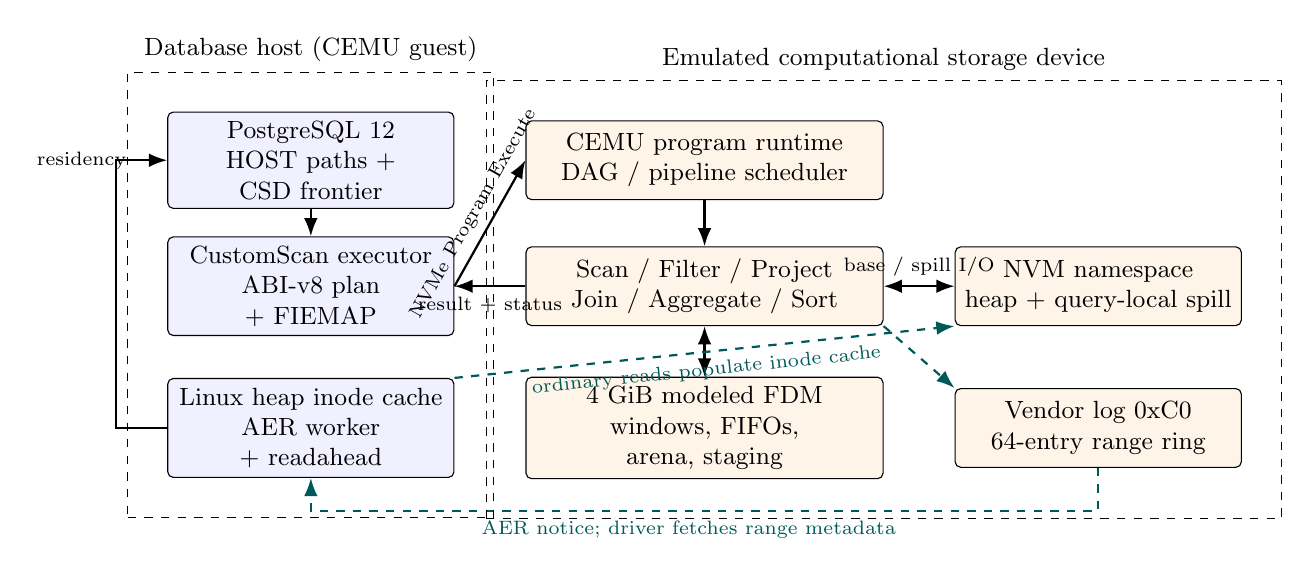
\begin{tikzpicture}[font=\small, >=Latex,
 box/.style={draw, rounded corners=2pt, align=center, minimum height=10mm},
 host/.style={box, fill=blue!6}, device/.style={box, fill=orange!9},
 flow/.style={->, thick}, hint/.style={->, dashed, thick, teal!70!black}]
\node[host, text width=34mm] (pg) at (0,2.0) {PostgreSQL 12\\HOST paths + CSD frontier};
\node[host, text width=34mm] (exec) at (0,0.4) {CustomScan executor\\ABI-v8 plan + FIEMAP};
\node[host, text width=34mm] (cache) at (0,-1.4) {Linux heap inode cache\\AER worker + readahead};
\node[device, text width=43mm] (runtime) at (5,2.0) {CEMU program runtime\\DAG / pipeline scheduler};
\node[device, text width=43mm] (ops) at (5,0.4) {Scan / Filter / Project\\Join / Aggregate / Sort};
\node[device, text width=43mm] (fdm) at (5,-1.4) {4 GiB modeled FDM\\windows, FIFOs, arena, staging};
\node[device, text width=34mm] (flash) at (10,0.4) {NVM namespace\\heap + query-local spill};
\node[device, text width=34mm] (log) at (10,-1.4) {Vendor log 0xC0\\64-entry range ring};
\draw[flow] (pg) -- (exec);
\draw[flow] (exec.east) -- node[above, sloped, font=\scriptsize]{NVMe Program Execute} (runtime.west);
\draw[flow] (runtime) -- (ops);
\draw[flow, <->] (ops) -- (fdm);
\draw[flow, <->] (ops) -- node[above, font=\scriptsize]{base / spill I/O} (flash);
\draw[flow] (ops.west) -- node[below, font=\scriptsize]{result + status} (exec.east);
\draw[hint] (ops.south east) -- (log.north west);
\draw[hint] (log.south) -- ++(0,-.55) -| node[pos=.26, below, font=\scriptsize]{AER notice; driver fetches range metadata} (cache.south);
\draw[flow] (cache.west) -- ++(-.65,0) |- node[pos=.7, left, font=\scriptsize]{residency} (pg.west);
\draw[hint] (cache.north east) -- node[below, sloped, font=\scriptsize]{ordinary reads populate inode cache} (flash.south west);
\node[draw, dashed, fit=(pg)(exec)(cache), inner sep=5mm, label=above:{Database host (CEMU guest)}] {};
\node[draw, dashed, fit=(runtime)(ops)(fdm)(flash)(log), inner sep=5mm, label=above:{Emulated computational storage device}] {};
\end{tikzpicture}
}
\caption{CPU-based architecture. PostgreSQL composes operator and I/O requests
through the SNIA API; the library schedules application-specified batch
dependencies. FEMU maps individual requests to storage or CPU compute units.
AER-driven inode reads produce host cache state that feeds later placement.}
\Description{PostgreSQL planner and application orchestrator call a SNIA
library and FEMU adapter. Device CPU functions share device buffers and work
memory. An AER log triggers host cache reads and residency feedback.}
\label{fig:architecture}
\end{figure*}

Figure~\ref{fig:architecture} separates four responsibilities. PostgreSQL
parses and optimizes SQL, selects execution locations, and constructs
application-specific operator descriptors. The application executor allocates
buffers and assembles I/O and compute requests. The SNIA library manages
handles, dependency-aware execution, and completion notification. The FEMU
plugin maps these requests to NVMe commands and device CPU execution.

The SQL layer remains outside the generic storage interface. A scan descriptor
specifies column types, needed attributes, predicates, and physical extents.
A join descriptor specifies keys and join kind. These structures reside in
application-provided buffers; they are not additions to the standard API.
An operator consumes its own descriptors and produces a documented batch
layout for the next operator.

A typical query has a preparation phase, a streaming phase, and a result
phase. Preparation opens the device, resolves functions, allocates AFDM
(application-allocated function data memory), and assigns a query work-memory
budget. Streaming loads input directly from NVM into AFDM and advances
compute batches. Blocking operators retain private state across invocations.
The result phase drains source functions, copies final result batches to
PostgreSQL, and releases operator state and buffers. Intermediate rows remain
inside device memory or spill storage throughout a device fragment.

\section{SNIA Interface and Application Orchestration}
\label{sec:api}
\subsection{Public API and Backend Separation}
Applications include \texttt{cs.h} and link \texttt{libsnia}. The public layer
handles discovery, device access, AFDM allocation, storage requests, compute
requests, batches, and events. A dynamically loaded FEMU adapter implements
device-specific operations. The application selects resources through
handles rather than encoding an NVMe command layout in each operator call.
Table~\ref{tab:api} shows the main interface groups used by SQL execution.

\begin{table}[t]
\caption{Application operations and representative SNIA APIs.}
\label{tab:api}
\small
\begin{tabular}{@{}p{.29\columnwidth}p{.65\columnwidth}@{}}
\toprule
Purpose & Representative calls \\
\midrule
Discover / open & \texttt{csQueryCSxList}, \texttt{csOpenCSx} \\
Inspect resources & \texttt{csQueryDeviceProperties} \\
Allocate / transfer & \texttt{csAllocMem}, \texttt{csQueueCopyMemRequest} \\
Load / identify CSFs & \texttt{csCSFDownload}, \texttt{csConfig}, \texttt{csGetCSFId} \\
Internal storage I/O & \texttt{csQueueStorageRequest} \\
Invoke computation & \texttt{csQueueComputeRequest} \\
Compose dependencies & \texttt{csAllocBatchRequest}, \texttt{csConfigureBatchEntry} \\
Submit / await & \texttt{csQueueBatchRequest}, \texttt{csPollEvent} \\
\bottomrule
\end{tabular}
\end{table}

The public library snapshots request descriptions and retains references to
functions and memory until completion. This separates descriptor lifetime
from buffer lifetime: configuring a request does not copy the underlying
AFDM contents. A producer and consumer can share one AFDM handle, allowing
intermediate data to stay on the device.

The backend translates AFDM references to native memory ranges and maps
compute calls to function invocation. Storage LOAD moves NVM ranges into
AFDM; STORE moves AFDM ranges back to NVM. Discovery and resource queries
report memory capacity and available compute resources to the application.
Callbacks or events deliver completion without a query-specific proxy process.

\subsection{Application-Defined Pipelines}
A batch specifies SERIAL, PARALLEL, or dependency-aware HYBRID execution.
For example, four input partitions can each use
\texttt{LOAD $\rightarrow$ Scan $\rightarrow$ Filter $\rightarrow$ sink}.
The branches are independent, but every sink depends on its own input load
and compute predecessors. The application supplies these dependencies;
the library dispatches ready requests subject to reported CU concurrency.

A blocking boundary uses sink/source functions. Repeated sink calls consume
input batches and retain state through an opaque handle. Once all sinks
finish, the application connects their handles to a source and downstream
operators. A source can produce one bounded output chunk per invocation.
For sorting followed by aggregation, the application first submits parallel
LOAD/sort-sink branches, then repeatedly submits
\texttt{sort-source $\rightarrow$ aggregate} until end of stream.
There is no need to copy sorted rows to the host between these calls.

The PostgreSQL executor derives pipeline boundaries and readiness from its
physical plan. A shared hash build completes before parallel probe requests
start. Completed execution slots immediately accept new work rather than
waiting for all slots to finish a fixed round. The same buffers can be
reused by later pipelines after their consumers complete. This places
scheduling policy with the application while allowing the library to manage
request dependencies uniformly.

\subsection{Reentrant Spill Requests}
A device function can suspend work when it needs internal storage I/O. Its
completion value requests STORE, LOAD, or FREE and identifies the amount or
token involved. The FEMU adapter carries out the storage operation and
reenters the same function with the completion token. The function's private
state records its continuation. A logical batch node completes only after
the function returns a normal result, so successors do not observe an
unfinished spill operation.

This division preserves application control of the operator graph without
requiring the application to interpret each operator's intermediate rows.
The API library schedules logical dependencies; the backend handles device
I/O continuation; the CSF owns its algorithmic state.

\section{Composable SQL Operators on Device CPUs}
\label{sec:operators}
\subsection{Scanning and Vectorized Expressions}
The application maps PostgreSQL heap files to physical extents and submits
internal LOAD requests. Scan functions decode PostgreSQL pages and emit
column batches, NULL masks, and selection vectors \cite{pgstorage}.
Projection pruning decodes only attributes required by predicates or
consumers. Deferred decoding avoids materializing expensive numeric or
string values for rows already rejected by simpler conditions.

The CPU kernels process bounded vectors, with 256-row batches as a useful
implementation unit. SIMD comparisons and arithmetic handle compatible
integer lanes; exact wider arithmetic handles decimal operations that need
it. A shared expression representation covers arithmetic, comparisons,
Boolean logic, CASE, LIKE, substring, and date extraction. NULL and decimal
precision travel with the values through each operator boundary.

Execution throughput depends on CPU resources, vector width, memory access,
CU concurrency, and storage I/O.
The application can fuse compatible scan/filter/projection work in one
function or compose separate functions over shared AFDM.

\subsection{Shared Memory Budgets}
The design distinguishes data-transfer buffers from private algorithm state.
AFDM holds raw input, column batches, control records, output, and reusable
spill I/O buffers. Hash tables, sort runs, cursors, and aggregate state use
a shared work-memory allocator. Per-query root contexts and operator child
contexts charge allocations to the same global pool.

Let $M_A$ denote AFDM reservations and $M_W$ the shared algorithm budget.
For $k$ concurrent operators, admission requires
\begin{equation}
 M_A \leq M_{\mathrm{AFDM}},\qquad
 \sum_{i=1}^{k} M_{W,i} \leq M_W.
\end{equation}
The application chooses chunk size and concurrent slots using both budgets.
A work-memory limit is a shared query constraint, not a fresh allocation for
every CU. Spill space is accounted separately on NVM. This avoids turning
parallel execution into unbounded memory replication.

\subsection{Join, Aggregate, and External Sort}
Hash joins retain a build table and stream probe batches, supporting INNER,
LEFT, SEMI, and ANTI semantics with residual predicates. When build state
exceeds its quota, the operator preserves consumed input and transitions to
an external path. Sorting both inputs and merging permits bounded progress;
duplicate-key groups can spill as well. Native index lookup can accelerate
parameterized integer-key joins when the application selects that access
path. The choice belongs to the SQL layer, not to the generic API library.

Aggregation consumes batches through sink functions and emits groups through
sources. SUM and COUNT maintain exact state; AVG retains sum and count until
finalization. Hash aggregation serves suitable keys and aggregate types;
ordered aggregation consumes sorted groups. Large state can be spilled and
combined through external sorting. DISTINCT retains its key and NULL rules
across run boundaries. HAVING and final projections follow aggregation in
the application-defined pipeline.

External Sort generates memory-resident runs until its budget is exhausted,
then stores runs in bounded Flash blocks. A source merges resident and
spilled runs with a memory-admitted fan-in, emits bounded output chunks,
and releases consumed storage. Intermediate merge passes are introduced only
when the available cursor memory cannot admit all runs. Exact LIMIT/OFFSET
bounds can truncate work where semantics allow. The source passes output
directly to the next device operator, avoiding an unnecessary final
write/read or host round trip.

\begin{table}[t]
\caption{SQL execution responsibilities within the application framework.}
\label{tab:operators}
\small
\begin{tabular}{@{}p{.25\columnwidth}p{.69\columnwidth}@{}}
\toprule
Operator family & CPU CSF behavior \\
\midrule
Scan / access & Heap decode, projected columns, optional index traversal \\
Filter / Project & Selection vectors, SIMD, exact scalar expressions \\
Join & Shared build, streamed probes, external fallback, join-kind semantics \\
Aggregate & Sink/source state, grouped/global reduction, DISTINCT \\
Sort / Limit & Bounded runs, external merge, chunked output, Top-N \\
Subquery / CTE & Application dependencies, scalar parameters, shared state \\
\bottomrule
\end{tabular}
\end{table}

The complete query is composed from these operator families
(Table~\ref{tab:operators}). Subquery decorrelation exposes joins and aggregate
branches to the same planning process. Reusable CTE or build state can have
multiple consumers, with ownership retained until the last consumer finishes.
Only a device fragment's final output crosses into the PostgreSQL executor.

\section{Asynchronous Host Cache Refill}
\label{sec:cache}
\subsection{From Device Scan to Host Inode}
A CSD scan reports the ranges it has consumed using a vendor event and range
log. An entry identifies relation, logical offset, length, namespace,
physical range, and execution generation. The notification informs the host
that cache-refill opportunities exist. The NVMe driver fetches the log and
resolves each range to a registered PostgreSQL heap segment.

AER is the control path. Data reaches the host through ordinary reads or
inode readahead. This distinction is essential because a physical read
against a block-device inode does not populate the corresponding heap-file
inode cache. The application registers relation identifiers and open segment
references before computation; the driver uses those references to direct
the reads to the correct mapping.

Adjacent ranges can be coalesced to amortize notification overhead. Sequence
and generation fields avoid repeated or stale work across query executions.
A final marker identifies the end of a refill stream, while completion
counters distinguish ranges announced, reads submitted, and pages actually
ready in cache. Queries normally proceed asynchronously; experiments can
wait for completion to isolate the effect of a fully populated cache.

\subsection{Overlap and Resource Control}
\begin{figure*}[t]
\centering
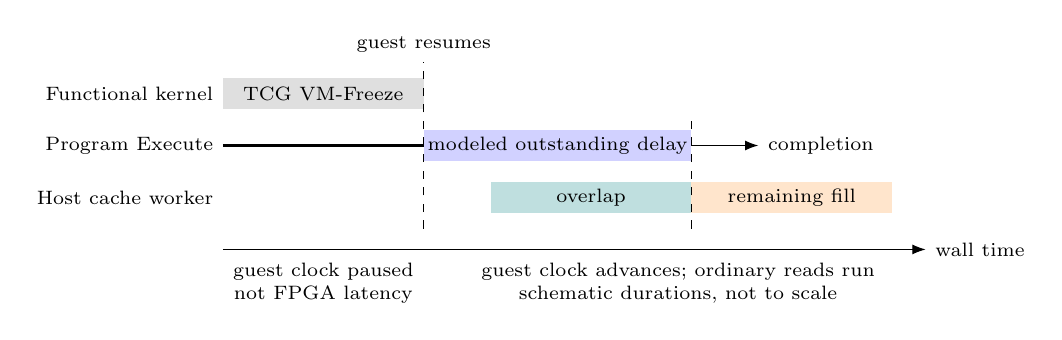
\begin{tikzpicture}[font=\scriptsize, >=Latex, x=.85cm, y=.66cm]
\node[anchor=east] at (0,2) {Functional kernel};
\node[anchor=east] at (0,1) {Program Execute};
\node[anchor=east] at (0,0) {Host cache worker};
\fill[gray!25] (0,1.7) rectangle (3,2.3);
\node at (1.5,2) {TCG VM-Freeze};
\draw[thick] (0,1) -- (3,1);
\fill[blue!18] (3,.7) rectangle (7,1.3);
\node at (5,1) {modeled outstanding delay};
\draw[->] (7,1) -- (8,1) node[right] {completion};
\fill[teal!25] (4,-.3) rectangle (7,.3);
\fill[orange!20] (7,-.3) rectangle (10,.3);
\node at (5.5,0) {overlap};
\node at (8.5,0) {remaining fill};
\draw[dashed] (3,-.6) -- (3,2.6) node[above] {guest resumes};
\draw[dashed] (7,-.6) -- (7,1.5);
\draw[->] (0,-1) -- (10.5,-1) node[right] {wall time};
\node[align=center] at (1.5,-1.65) {guest clock paused\\not FPGA latency};
\node[align=center] at (6.8,-1.65) {guest clock advances; ordinary reads run\\schematic durations, not to scale};
\end{tikzpicture}

\caption{Intended overlap for application-orchestrated CPU execution. Range
notifications permit host reads while later device batches execute. Refill
may continue after a query finishes; the next plan observes actual residency.}
\Description{A host submits CPU CSF batches. Device scan ranges generate AER
notifications, host reads overlap later device computation, and the next
query samples the resulting cache residency.}
\label{fig:timeline}
\end{figure*}

Figure~\ref{fig:timeline} illustrates the overlap opportunity. A device batch
finishes scanning one range while other CPU computation or later batches
remain in flight. The host processes its range notification and starts reads
without waiting for the whole query. Buffer consumption and operator
execution continue through the application scheduler.

Refill uses available host-interface bandwidth but also creates additional
storage traffic. It should yield to foreground result transfer and can be
rate-limited or curtailed under memory pressure. Its effect should therefore
be measured as both current-query overhead and subsequent-query benefit.
A best-effort event loss sacrifices a warming opportunity without changing
SQL results. The planner consumes observed resident pages, rather than
assuming that every notified range was successfully cached.

\section{Cache-Aware Node-Level Placement}
\label{sec:placement}
\subsection{Execution Alternatives}
The optimizer considers a host state $H(v)$ and device-resident alternatives
$D(v)$ for each operator $v$. The decision is made bottom-up at node
granularity. A single compatible node, a connected subtree, or the complete
plan can execute on the CSD. An upper device node requires device-resident
inputs; host intermediates are not uploaded back to the CSD. Each dataflow
path can therefore transition from CSD to HOST once.

This restriction aligns planning with the data path. A device scan can feed
a device join and aggregate, then return a small result to a host sort.
Alternatively, a cached scan and all its ancestors can remain on the host.
The application translates the selected device fragments into SNIA requests
and dependencies; placement does not require a device-side query scheduler.

\subsection{Cost Model and Dynamic Program}
For each physical alternative, local device cost includes CPU work and
storage movement:
\begin{equation}
 \ell_D(v)=C_{\mathrm{CPU}}(v)+C_{\mathrm{I/O}}(v)
                          +C_{\mathrm{spill}}(v).
\end{equation}
CPU cost is estimated from measured scan/decode, expression, hash, aggregate,
and sort throughput at the chosen CU concurrency. Spill cost includes both
writes and replay reads. A device-to-host boundary adds request setup and
result transfer, so the recurrence is
\begin{align}
 D(v)&=\ell_D(v)+\sum_{u\in\mathrm{child}(v)}D(u),\\
 X(v)&=D(v)+C_{\mathrm{setup}}+\widehat{B}_v/W_{\mathrm{return}},\\
 H(v)&=\ell_H(v)+\sum_{u\in\mathrm{child}(v)}\min\{H(u),X(u)\},\\
 C_{\mathrm{root}}&=\min\{H(v),X(v)\}.
\label{eq:dp}
\end{align}
Here $X(v)$ materializes the device result for HOST and $\widehat{B}_v$ is
expected serialized output size. Internal device edges reuse buffers and do
not repeatedly pay result transfer. Actual planning retains alternative
orders, algorithms, and physical properties rather than a single scalar
per state.

For a relation with $p_r$ pages and observed resident fraction $h_r$, the
host scan I/O component is
\begin{equation}
 C_{H,\mathrm{scan}}(r)=p_r[(1-h_r)c_{\mathrm{storage}}
                                  +h_r c_{\mathrm{cached}}].
\end{equation}
Cache sampling uses the heap segments' actual residency. Refills from an
earlier device query raise $h_r$ and can change the next query's placement.
This connects cache production to the planning objective without awarding
speculative benefits for data that is not yet resident.

\subsection{Candidate Retention and Resource Admission}
A locally cheap HOST path can hide a device alternative whose output becomes
small after an upper aggregate. A private frontier preserves device-resident
candidates alongside the database's normal host paths. Join planning combines
surviving child alternatives; upper nodes consider every compatible input.
Dominance compares cost and resource demand only among candidates with
compatible ordering, dependencies, and semantic state.

Expected rows drive execution cost; a separate resource estimate checks
buffer and operator-state admission. Scan bounds derive from physical pages,
join bounds from input and join type, and LIMIT from the SQL bound. Grouping
uses conservative statistics with runtime memory checks. A large device
intermediate may remain useful to an upper device reducer even when returning
that intermediate to HOST would be expensive. Spill and return boundaries
are therefore evaluated independently.

\section{Evaluation}
\label{sec:evaluation}
The evaluation follows the four contributions in order: API composition,
complete operator execution, cache refill, and adaptive placement. We use
TPC-H Q1--Q22 at SF=1 as the initial workload \cite{tpch}, supplemented with
operator microbenchmarks and repeated query sequences.

\paragraph{Status of the reference results.}
The numerical figures below reuse the existing SF=1 companion-prototype
measurements as preliminary reference data. They guide experiment selection
and expected trends; final CPU/SNIA measurements will replace them. The five-way
ablation is specified here with unmeasured cells left open, rather than
inferred from those reference numbers.

\subsection{Configurations and Comparison Questions}
Table~\ref{tab:baselines} defines the five configurations. They share SQL,
data layout, CPU/CU allocation, memory budgets, and device bandwidth settings.
Offload-capable configurations use the same SNIA backend so the operator
comparison is not confounded by a different transport.

\begin{table*}[t]
\caption{Five-way comparison. Each added mechanism answers a separate
question; Filter-only is a restricted baseline, not a description of every
prior system.}
\label{tab:baselines}
\small
\begin{tabular}{@{}p{.14\textwidth}p{.24\textwidth}p{.06\textwidth}p{.09\textwidth}p{.35\textwidth}@{}}
\toprule
Configuration & Operator placement & Refill & Adaptive & Comparison purpose \\
\midrule
Host-only & All relational work on native PostgreSQL & No & No & Reference execution without offload \\
Filter-only & Device scan/filter; host joins, aggregates, sort & No & No & Benefit and limit of predicate offload \\
CSD-only & All supported relational work on device CPUs & No & No & Incremental value of complete operator chains \\
CSD + Cache Refill & Same forced-device placement as CSD-only & Yes & No & Cost and reuse benefit of cache population \\
Full system & Node-level HOST/CSD choices & Yes & Yes & Additional benefit of cache-aware placement \\
\bottomrule
\end{tabular}
\end{table*}

Host-only versus Filter-only isolates early row reduction. Filter-only versus
CSD-only measures whether joins and blocking operators avoid substantial
intermediate transfer. CSD-only versus CSD + Cache Refill must be compared
both for the first query and for later queries: refill can add traffic now
while saving I/O later. CSD + Cache Refill versus the full system isolates
placement, since their operator library and refill mechanism are identical.

\subsection{Setup and Measurement Protocol}
The final setup records host and device CPU resources, CU count, AFDM,
shared work memory, storage bandwidth, API request cost, and query memory
settings. A CU sweep uses 1, 2, and 4 concurrent device requests. Memory
experiments vary AFDM and work-memory limits separately; the example operator
library provides a 64 MiB work-memory setting as an initial pressure point.
The same total budget applies across CUs.

Cold-query experiments restart PostgreSQL and clear the host file cache
before every configuration sample. Warm and sequential experiments instead
retain cache across a specified query sequence, clearing only before the
sequence. All outputs are checked against Host-only. Repeated measurements
report median, dispersion, and total query-sequence completion time.
End-to-end latency is the primary metric; CPU time, per-CSF time, bytes
transferred, refill completion, memory peaks, and spill traffic explain it.
Overlapping per-request times are not summed as query latency.

\begin{table*}[t]
\caption{Main results template for the CPU/SNIA implementation. Dashes mark
measurements to be filled; they do not denote zero. All configurations run
the same queries and sequence definitions.}
\label{tab:resultslots}
\small
\resizebox{\textwidth}{!}{%
\begin{tabular}{@{}lrrrrr@{}}
\toprule
Metric & Host-only & Filter-only & CSD-only & CSD + Cache Refill & Full system \\
\midrule
Cold Q1--Q22 total latency (s) & \pending & \pending & \pending & \pending & \pending \\
Warm Q1--Q22 total latency (s) & \pending & \pending & \pending & \pending & \pending \\
Repeated-query sequence latency (s) & \pending & \pending & \pending & \pending & \pending \\
Mixed-query sequence latency (s) & \pending & \pending & \pending & \pending & \pending \\
Host-interface data traffic (GiB) & \pending & \pending & \pending & \pending & \pending \\
Device spill read + write (GiB) & \pending & \pending & \pending & \pending & \pending \\
Peak query memory (MiB) & \pending & \pending & \pending & \pending & \pending \\
Correct query outputs / 22 & \pending & \pending & \pending & \pending & \pending \\
\bottomrule
\end{tabular}}
\end{table*}

Table~\ref{tab:resultslots} is the main result matrix to fill. Per-query bars
will show the five configurations normalized to Host-only. Separate sequence
plots will show cumulative completion time and measured cache residency, so
cache production and location changes are visible together.

\subsection{API and Complete-Operator Evaluation}
The interface microbenchmarks measure allocation, compute request latency,
event completion, and SERIAL versus HYBRID batches. A composed
LOAD--sort-sink / sort-source--aggregate workload tests that intermediate
rows stay inside the device and that parallel branches share one memory
budget. It also separates useful CPU work from request and continuation cost.

For TPC-H, Filter-only and CSD-only should be compared by selectivity,
intermediate bytes returned, and the number of host blocking operators.
Q6 represents a simple scan/reduction chain; Q3 and Q5 exercise joins and
aggregation; Q18 exercises grouping, joins, and ordering. The purpose is to
identify when a complete fragment is better than returning filtered rows,
not to assume that more offload always wins.

Existing reference profiles illustrate the state-management questions.
Streaming Q1 and Q6 aggregation consume 29 batches and record small operator
state peaks of 2,528 and 134 bytes. A forced 1 MiB join replay returns count
299,808 with a 750,240-byte recorded state peak. A grouped replay returns
74,999 groups with 796,876 bytes of recorded state. These values motivate
separate reporting of buffers, private state, and spill; the CPU/SNIA operator
experiments will measure those categories directly.

\begin{figure}[t]
\centering
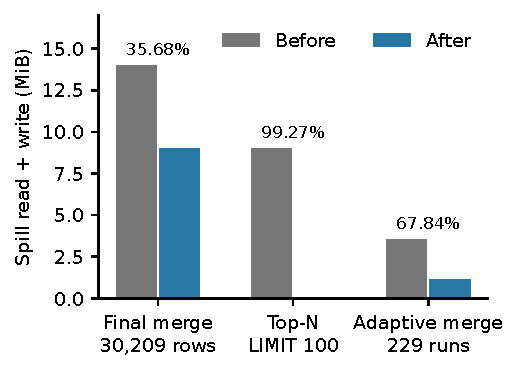
\includegraphics[width=\columnwidth]{figures/sf1_sort_io.pdf}
\caption{Preliminary SF=1 reference: three separate external-sort I/O
comparisons. Final output streaming, SQL Top-N, and wider merging motivate
CPU operator ablations; each pair has its own baseline.}
\Description{Paired bars compare spill traffic before and after final
streaming, Top-N, and adaptive merging in the reference data.}
\label{fig:sort}
\end{figure}

Figure~\ref{fig:sort} supplies reference points for the external-sort study.
Final merge-to-consumer streaming reduces spill traffic from 14,646,232 to
9,420,282 bytes. A LIMIT 100 query needs 69,190 bytes against the latter
unbounded reference. In a separate 229-run test, wider merging reduces traffic
from 3,680,832 to 1,183,632 bytes. The final CPU experiments will compare
matched SQL and budgets, including output streaming, Top-N, fan-in, and
work-memory sensitivity.

\subsection{Cache Refill: Immediate Cost and Future Benefit}
We use two complementary experiments. A controlled two-query experiment
first offloads a scan and then executes a forced-host query over the same
relation. Waiting for refill before the second query isolates achievable
cache benefit. A sequence experiment removes that wait and includes all
refill overhead in elapsed time, measuring whether asynchronous warming
improves the workload as a whole.

\begin{figure}[t]
\centering
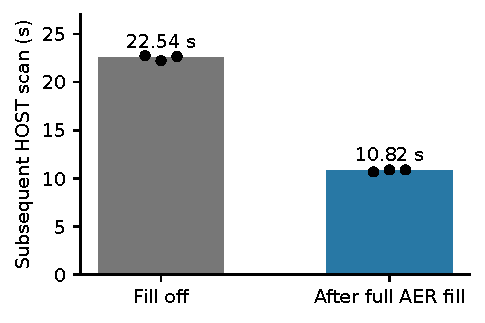
\includegraphics[width=\columnwidth]{figures/sf1_cache_benefit.pdf}
\caption{Preliminary reference for subsequent-query cache benefit. After
complete refill, the HOST count scan averages 10.82 s instead of 22.54 s;
dots represent the three archived samples.}
\Description{Bars and sample points compare a subsequent host scan with
refill disabled and after complete refill.}
\label{fig:cache}
\end{figure}

The reference two-query experiment returns 6,001,215 in both paths.
Subsequent HOST scan time averages 22,537.964 ms without refill and
10,818.313 ms after complete refill, a 2.0833 ratio
(Figure~\ref{fig:cache}). The completed range is 1,276,665,856 bytes across
two heap segments. A separate overlap experiment records 128 MiB completed
inside a roughly 1.218 s outstanding command window. These observations
motivate measuring completed refill bytes, first/last completion, and the
fraction overlapping useful device work.

For the final five-way comparison, CSD + Cache Refill and CSD-only use exactly
the same forced-device plan. We report current-query overhead, next-query
latency, total sequence latency, extra NVM/host traffic, and cache residency.
A refill-rate sweep tests whether excessive warming competes with useful
computation or result transfer. Repeated scans and mixed query sequences
separate high reuse from cache pollution.

\subsection{Full System: Cache-Aware Placement}
\begin{figure*}[t]
\centering
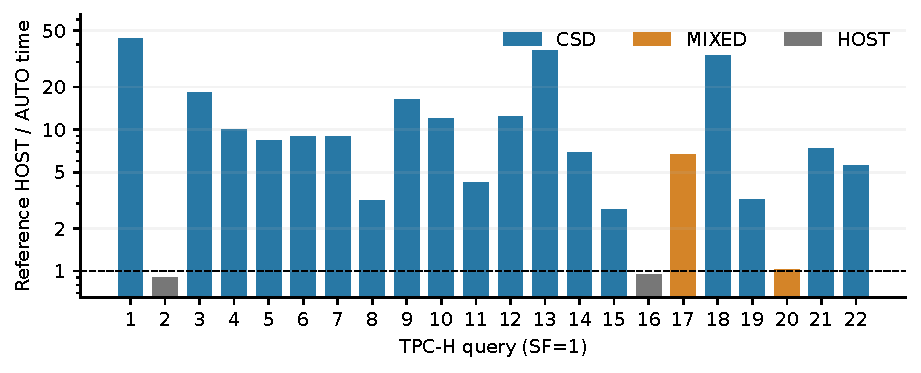
\includegraphics[width=.94\textwidth]{figures/sf1_auto_speedup.pdf}
\caption{Preliminary SF=1 placement reference. Colors identify complete CSD,
mixed, and HOST choices. The final evaluation will replace this two-path
reference with the five configurations in Table~\ref{tab:baselines}.}
\Description{Per-query reference time ratios show different host, device,
and mixed placements across the 22 TPC-H queries.}
\label{fig:placement}
\end{figure*}

The reference placement run chooses 18 complete CSD plans, two mixed plans,
and two HOST plans. Total reference times are 183,019.742 ms for AUTO and
825,114.403 ms for HOST, an aggregate ratio of 4.5083; the geometric mean of
per-query ratios is 6.9207 (Figure~\ref{fig:placement}). These values establish
an initial scale for the study, while the final five-way experiment isolates
the additional effect of the CPU/SNIA architecture and refill-aware choice.

The placement experiment sweeps measured resident fraction from cold to hot
and records the chosen location at each node. We compare the full system
against forced CSD + Cache Refill, a cache-oblivious placement variant, and
an offline best-of-configurations reference. The offline reference is an
analysis bound, not a deployable optimizer.

A mixed-query sequence starts with a selective offloaded query, then submits
queries over overlapping and disjoint relations. We track cumulative time,
cache-resident bytes, device spill, and the locations selected at successive
planning points. This directly tests the intended chain: complete device
execution creates refill opportunities, refill changes host scan cost, and
node-level planning uses the changed cost. Performance on unrelated queries
checks whether the same refill also harms cache capacity.

\section{Design Tradeoffs}
The architecture deliberately exposes composition to the application. This
avoids embedding SQL scheduling policy in generic device services and allows
non-SQL applications to use the same API. Its cost is more visible request
and buffer management in the executor. Fusing short chains and reusing batch
descriptions amortize that cost without changing the public interface.

CPU CUs provide flexible operators, vectorization, and shared state, but
operator concurrency must respect both work memory and storage bandwidth.
The application should increase parallelism only while useful work grows;
spilling several concurrent builds can be worse than serializing them.
Memory and CU sensitivity experiments therefore accompany the main results.

Refill trades a portion of the transfer reduction for future cache reuse.
The system observes its effect at later planning points rather than assuming
future reuse is guaranteed. Refill priority, cancellation, cache pressure,
and range lifetime are natural policy dimensions to study after the main
operator/refill/placement comparison.

\section{Related Work}
\paragraph{Near-storage query execution.}
Ibex demonstrates richer SQL offload than simple filtering, including GROUP
BY \cite{ibex}. PushdownDB explores the capabilities and limits of cloud
storage computation \cite{pushdowndb}. Trinity integrates database execution
with near-data acceleration \cite{trinity}, while NASCENT specializes
near-storage sorting \cite{nascent}. These systems motivate operator coverage
and locality. Our design emphasizes composable CPU functions through SNIA,
application-controlled execution, and explicit host cache replenishment.
Filter-only serves as a useful restricted baseline without reducing these
systems to that baseline.

\paragraph{Caching and adaptive pushdown.}
FlexPushdownDB combines cached segments with pushed-down work through
separable operators \cite{fpdb}. Subsequent adaptive-pushdown work also
considers storage-side resource pressure \cite{adaptivepushdown}. Thus the
joint importance of caching and placement is established. Our focus is the
locally attached CSD setting: device scans actively expose ranges for host
inode-cache refill, and node-level planning consumes the resulting residency.
The difference lies in the refill mechanism and its integration with complete
operator fragments over a standard interface.

\paragraph{Interfaces and emulation.}
SNIA supplies the common application interface \cite{snia}; FEMU supplies the
extensible SSD emulation foundation \cite{femu}. \sys{} connects the interface
to CPU-based SQL functions and application-controlled pipelines. This
separation permits interface, operator, and planning improvements to be
studied independently through the same request path.

\section{Conclusion}
\sys{} organizes computational-storage query execution around four connected
steps: a standard interface, composable CPU SQL operators, asynchronous host
cache refill, and cache-aware node-level placement. The application controls
execution through SNIA batches while intermediate data remains inside the
device. Cache refill turns completed scans into future host opportunities,
and the optimizer uses observed residency to choose the next execution
location. The five-configuration evaluation separates the benefit of each
step and provides the structure for completing the CPU-based implementation
and measurements.

\bibliographystyle{ACM-Reference-Format}
\bibliography{references}
\end{document}
